%\documentclass[12pt,a4paper]{report}
\documentclass[12pt,a4paper,oneside,onecolumn,openright]{book}
% set the document language
\usepackage[english]{babel}
% set the encoding used by your editor here (default is utf8)
\usepackage[utf8]{inputenc}
\usepackage[T1]{fontenc}

% math packages
\usepackage{amsmath}
\usepackage{amssymb}
% page margins settings
\usepackage[inner=3cm,outer=2.5cm,top=3cm,bottom=2.5cm]{geometry}
%\usepackage{indentfirst}

% other packages
\usepackage{array}
\usepackage{subfigure}
\usepackage{graphicx}
\usepackage{verbatim}
\usepackage{listings}
\usepackage{url}
\usepackage[hidelinks]{hyperref}
\usepackage{algorithm}
\usepackage{algpseudocode}
% custom colors
\usepackage{color}
\definecolor{light-gray}{gray}{0.96}
\definecolor{cyan}{RGB}{230,230,255}
\definecolor{dkgreen}{rgb}{0,0.6,0}
\definecolor{gray}{rgb}{0.5,0.5,0.5}
\definecolor{mauve}{rgb}{0.58,0,0.82}

% environment for bash code
\lstset{ %
  language=bash,                % the language of the code
  basicstyle=\footnotesize,           % the size of the fonts that are used for the code
  numbers=left,                   % where to put the line-numbers
  numberstyle=\footnotesize,          % the size of the fonts that are used for the line-numbers
  stepnumber=1,                   % the step between two line-numbers. If it's 1, each line
                                  % will be numbered
  numbersep=5pt,                  % how far the line-numbers are from the code
  backgroundcolor=\color{white},      % choose the background color. You must add \usepackage{color}
  showspaces=false,               % show spaces adding particular underscores
  showstringspaces=false,         % underline spaces within strings
  showtabs=false,                 % show tabs within strings adding particular underscores
%  frame=single,                   % adds a frame around the code
  rulecolor=\color{black},        % if not set, the frame-color may be changed on line-breaks within not-black text (e.g. commens (green here))
  tabsize=2,                      % sets default tabsize to 2 spaces
  captionpos=b,                   % sets the caption-position to bottom
  breaklines=true,                % sets automatic line breaking
  breakatwhitespace=false,        % sets if automatic breaks should only happen at whitespace
  title=\lstname,                   % show the filename of files included with \lstinputlisting;
                                  % also try caption instead of title
  numberstyle=\tiny\color{gray},        % line number style
  keywordstyle=\textbf,          % keyword style
  commentstyle=\color{dkgreen},       % comment style
%  stringstyle=\color{mauve},         % string literal style
  escapeinside={\%*}{*)},            % if you want to add a comment within your code
  morekeywords={*,...,insert,-}               % if you want to add more keywords to the setù
}

% environment for python code
\lstset{
language=Python,
breaklines=true,
breakatwhitespace=true ,
backgroundcolor=\color{light-gray}
}

\lstset{
  basicstyle=\ttfamily,
  mathescape
}
% appendices package
%\usepackage{appendix}
% set Appendix name used in the toc
%\renewcommand{\appendixtocname}{Appendice}

% interline
\linespread{1.5}
% set numbers for subsections and show them in the toc
\setcounter{tocdepth}{3}
\setcounter{secnumdepth}{3}

% layout package, style and settings
\usepackage{fancyhdr}
\pagestyle{fancy}

\fancypagestyle{mainmatter}{%
		\fancyhf{}
		\fancyhead{}
		\fancyhead[LE,RO]{\thepage}
		\fancyhead[LO]{\footnotesize{\leftmark}}
		\fancyhead[RE]{\footnotesize{\rightmark}}
		\fancyfoot{}
		\addtolength{\headwidth}{\marginparsep}
		\addtolength{\headheight}{2.5pt}
		\renewcommand{\headrulewidth}{0.3pt}
		\renewcommand{\footrulewidth}{0.0pt}
		}
\fancypagestyle{frontmatter}{%
		\fancyhf{}
		\fancyhead[LE]{\footnotesize{\MakeUppercase{\thepage}}}
		\fancyhead[RO]{\footnotesize{\MakeUppercase{\thepage}}}
		\fancyhead[RE,LO]{}
		\fancyfoot{}
		\addtolength{\headwidth}{\marginparsep}
		\addtolength{\headheight}{2.5pt}
		\renewcommand{\headrulewidth}{0.0pt}
		\renewcommand{\footrulewidth}{0.0pt}
		}


\usepackage{fancyhdr}
\pagestyle{fancy}
		\fancyhf{}
		\fancyhead{}
		\fancyhead[LE,RO]{\thepage}
		\fancyhead[LO]{\footnotesize{\leftmark}}
		\fancyhead[RE]{\footnotesize{\rightmark}}
		\fancyfoot{}
		\addtolength{\headwidth}{\marginparsep}
		\addtolength{\headheight}{2.5pt}
		\renewcommand{\headrulewidth}{0.3pt}
		\renewcommand{\footrulewidth}{0.0pt}

% empty pages have no numbers
\makeatletter
\def\cleardoublepage{\clearpage\if@twoside \ifodd\c@page\else
\hbox{}
  %Potresti voler togliere il commento dalla linea seguente
  %Questa pagina e' stata lasciata intenzionalmente vuota.
\thispagestyle{empty}
\newpage
\if@twocolumn\hbox{}\newpage\fi\fi\fi}
\makeatother

\begin{document}
\begin{titlepage}
\begin{center}
{
	  \vspace{\stretch{12}}

 		\huge{\bf Meal forecasting}}\\
		\vspace{3mm}
 		{\huge{\bf with capacitated vehicle routing}}\\
		\vspace{6mm}
		{\large{\bf Algoritmi di Ottimizzazione Exam Project}}

		\vspace{\stretch{6}}
		\end{center}

\vspace{40mm}
\par
\noindent
\begin{minipage}[t]{0.47\textwidth}
{\large{\bf Author:\\
    Lorenzo Rossi (matr. 183590)}}
\end{minipage}
\hfill
\begin{minipage}[t]{0.47\textwidth}\raggedleft
{\large{\bf Academic Year:\\
2022/2023}}
\end{minipage}

\end{titlepage}

\pagestyle{frontmatter}
\frontmatter

\setcounter{tocdepth}{2}
\tableofcontents

\setlength{\parindent}{12pt}
\setlength{\parskip}{1ex plus 0.5ex minus 0.2ex}
\mainmatter
\pagestyle{mainmatter}

% Import every section
% In this chapter we explain/discuss/describe/present...
% - Project description
% - Meal forecasting
% - Data generation
% - Vehicle Routing
%   + Details
%   + Subproblem
%   + Implementation
% - Results

\chapter{Project description}
\label{project-description}

The aim of this project is to address a delivery problem for a meal delivery company that operates across multiple cities and regions. The company has several distribution centers, and its first challenge is to forecast the meals that each center will need to produce for the upcoming week, based on historical data of meal purchases aggregated by week.
Once the meals are forecasted, the company's next crucial task is to distribute the necessary ingredients from a central depot to the distribution centers. The primary objective of this task is to minimize the distance traveled during transportation.
Overall, the project aims to streamline the meal delivery company's operations by forecasting meal requirements accurately and optimizing ingredient distribution, ultimately enhancing customer satisfaction and improving business efficiency.


The company demand data was provided by Edwin U Kannanaikkal~\cite{analyticsvidhya2020} on Kaggle with a DbCLv1.0 license.
To solve the forecasting task the project implements two metrics, one is a simple average of N previous weeks projected in the future, the other is a more complex integration of the popular library for forecasting, prophet~\cite{taylor2018forecasting}.
Additional data not provided in the original files, like meal ingredients and facility locations, have been generated using a mix of statistics and machine learning to be as plausible as possible.
Finally, different solvers for the VRPC problem have been tried, a polynomial one, one with subtour-elimination, and the last one implemented by column generation and a custom branch and price algorithm.

The rest of this report is divided as follows:
Chapter~\ref{meal-forecasting} explains our tactics for forecasting meal demands,
Chapter~\ref{data-generation} describes how we generated the data that was not included in our data source,
Chapter~\ref{vehicle-routing} presents our implementation of the VRPC solver,
Chapter~\ref{results} confronts the achieved results of the project.

\chapter{Meal Forecasting}
\label{meal-forecasting}

Based on the historical data of meal purchases aggregated by week, spanning 145 weeks for each center, the initial objective of this project is to forecast the quantity of each food item that every distribution center will require. This prediction will involve analyzing the demand trends for each food item across the different centers, and identifying any patterns or seasonality in the data. The accurate forecasting of meal orders for each center will enable the company to efficiently plan and allocate resources, ensuring that they can meet the anticipated demand and minimize waste.

\section{Details}
\label{meal-forecasting-details}
The first reference metric is to take the average of N previous weeks and project it into the future, this is both easy to implement and quite accurate.

The second approach involves utilizing the widely used library, Prophet~\cite{taylor2018forecasting}, to capture the seasonality and trends in the demand data and project them into the future. In order to simplify the problem, we did not consider other additional data such as pricing, product features, or promotions. Instead, we solely focused on the number of orders per week. While this simplified approach negatively impacted the performance and precision of the model, we decided that it was the best option given the project's time constraints.

Given the high quantity of meal-facility pairs to analyze, the project also implements a multi-processing optimization that splits the computation load across the present CPU cores.

\section{Results}
\label{meal-forecasting-results}
To compare the results we will divide the data between training and testing, after that we compare the Mean Square Error of the whole dataset for the various strategies. To offer a better interpretation, 9 randomly selected meal-facility pairs have been plotted.

The only hyper-parameter involved in the first strategy is the number of weeks to average the demand data. After conducting several manual trials, we optimized this parameter to three weeks.


\begin{figure}[tb]
    \centering
    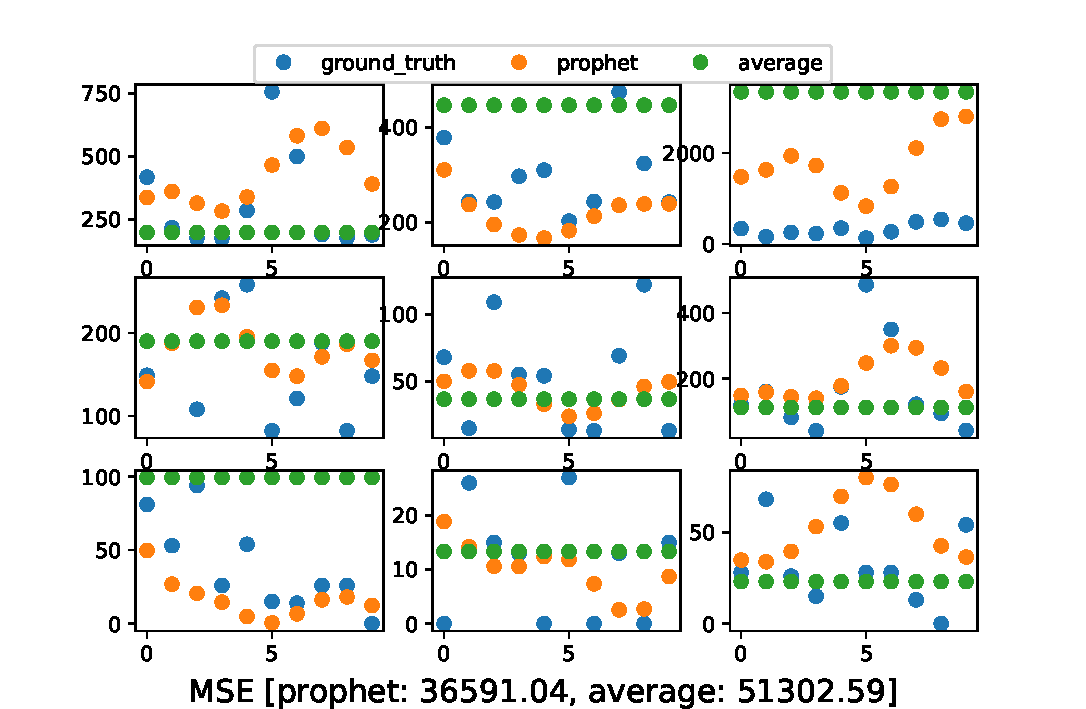
\includegraphics[width=1\columnwidth]{figures/meal_forecast_res_long.pdf}
    \caption{Meal Forecast results, 10 weeks}
  \label{fig:meal-forecast-res-long}
\end{figure}

As demonstrated in Figure~\ref{fig:meal-forecast-res-long}, the Prophet forecasting strategy outperforms the simple average approach in terms of accuracy, even without the use of auxiliary data. The Prophet model is able to capture the underlying trends and patterns in the demand data more effectively, and provide more accurate forecasts for future weeks. However, this advantage is not as significant when it comes to single-week forecasting.

\begin{figure}[tb]
    \centering
    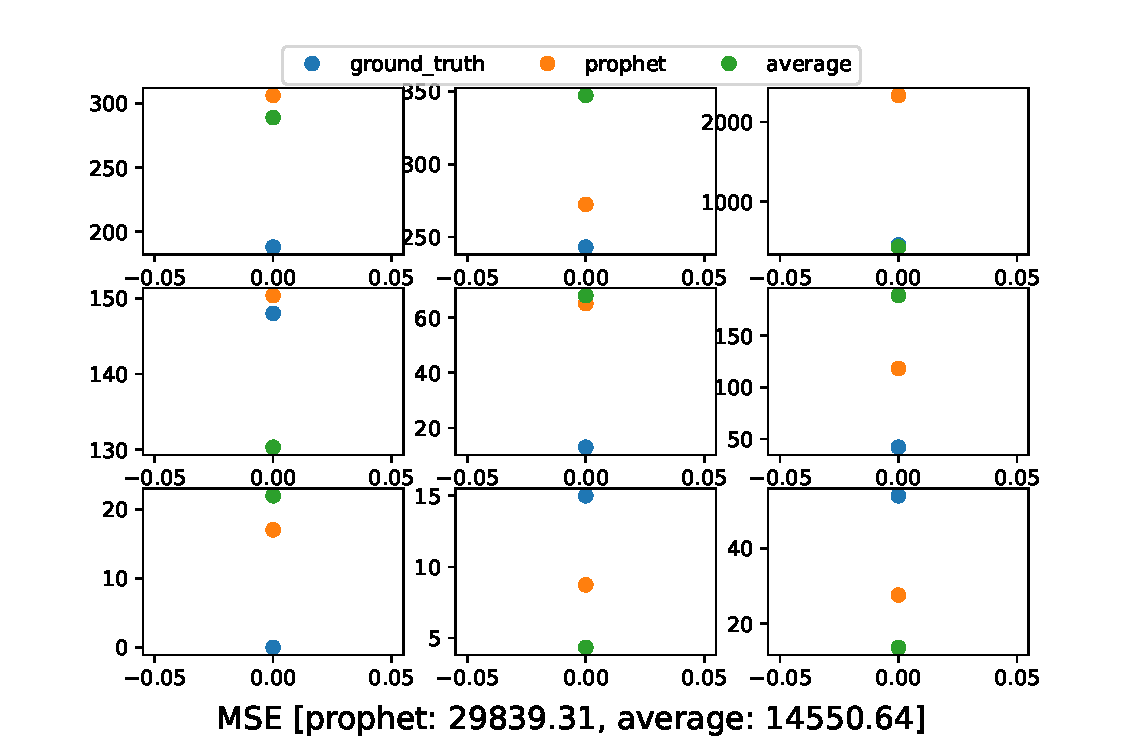
\includegraphics[width=1\columnwidth]{figures/meal_forecast_res_short.pdf}
    \caption{Meal Forecast results, 1 week}
  \label{fig:meal-forecast-res-short}
\end{figure}

However, as depicted in Figure~\ref{fig:meal-forecast-res-short}, when forecasting the outcome for a single week in advance, the average solution appears to provide better results. Although this could be attributed to inadequate utilization of the library or the presence of data outliers, we opted to proceed with the data that produced lower error since that part falls out of the project scope.

\chapter{Data Generation}
\label{data-generation}

The obtained data solely included information about meal orders, without any additional details about the distribution centers' locations or the ingredients incorporated in each meal. To effectively model the VRPC step, additional data was required. To address this data gap, both machine learning and statistical methodologies were utilized to generate a suitable dataset. The generation process utilized the hints provided in the original dataset to create data that was as plausible as possible.

Section~\ref{datagen-ingredient-composition} outlines the methodology utilized to generate a realistic ingredient list for each meal,
Section~\ref{datagen-distribution-center-locations} details the approach employed to randomly generate distribution center locations.

\section{Ingredient composition}
\label{datagen-ingredient-composition}
In order to generate the ingredient composition for each meal, we employed the use of ChatGPT, a sophisticated language model that is capable of generating text based on a given prompt. We sent the name for each meal and we asked how many grams of each ingredients are required, in order to ensure the accuracy and plausibility of the generated data, we implemented a human supervision step.

While the generated data did contain some errors, expecially in the weight of the ingredients, the supervisor could easily find and correct these, producing an high quality, mostly plausible ingredient list directly in CSV format. The following paste will contain an example of the generated data:


\begin{verbatim}
    meal_id,ingredient,weight_grams
    Pasta al Pesto,Pasta,100
    Pasta al Pesto,Basil Pesto,50
    Pasta al Pesto,Parmesan Cheese,20
    Pasta al Pesto,Pine Nuts,20
    Pasta al Pesto,Garlic,10
    Chicken Rice Bowl,Chicken,200
    Chicken Rice Bowl,White Rice,150
    Chicken Rice Bowl,Red Bell Pepper,50
    Chicken Rice Bowl,Cucumber,50
    Chicken Rice Bowl,Carrot,50
    Chicken Rice Bowl,Onion,20
    Chicken Rice Bowl,Soy Sauce,15
    Chicken Rice Bowl,Honey,10
\end{verbatim}

\section{Distribution center locations}
\label{datagen-distribution-center-locations}
The original data provides only partial information about the location of each facility, specifying only the city and region through anonymized IDs. Despite this limitation, we use the available data to generate plausible location positions for the centers. Instead of generating random positions for the centers directly, we first generate regions, then cities, and finally centers. This hierarchical approach enables us to use the known city and region information to inform the positions of the centers by relative positioning.

To ensure that the generated locations are feasible, we have implemented two additional constraints. Firstly, we ensure that the regions, cities, and centers are a minimum distance apart. If this criterion is not met, the positions are regenerated until the minimum distance is achieved. Secondly, we sample the distribution of centers from a normal distribution, with the variance varying based on the size of the city they are located in. This means that larger cities have more sparse facilities, while smaller cities have facilities located closer to their center.

The central depot is located using a similar method to that used for the centers. However, instead of choosing a specific city for the depot, we randomly select a city from among the available options, with a bias towards larger cities. This ensures that the central depot is strategically placed to enable efficient distribution to the centers located throughout the region.

The resulting distribution can be visualized in Figure~\ref{fig:center_locations}, depicting both regions, cities, centers and the central Depot.


\begin{figure}[tb]
    \centering
    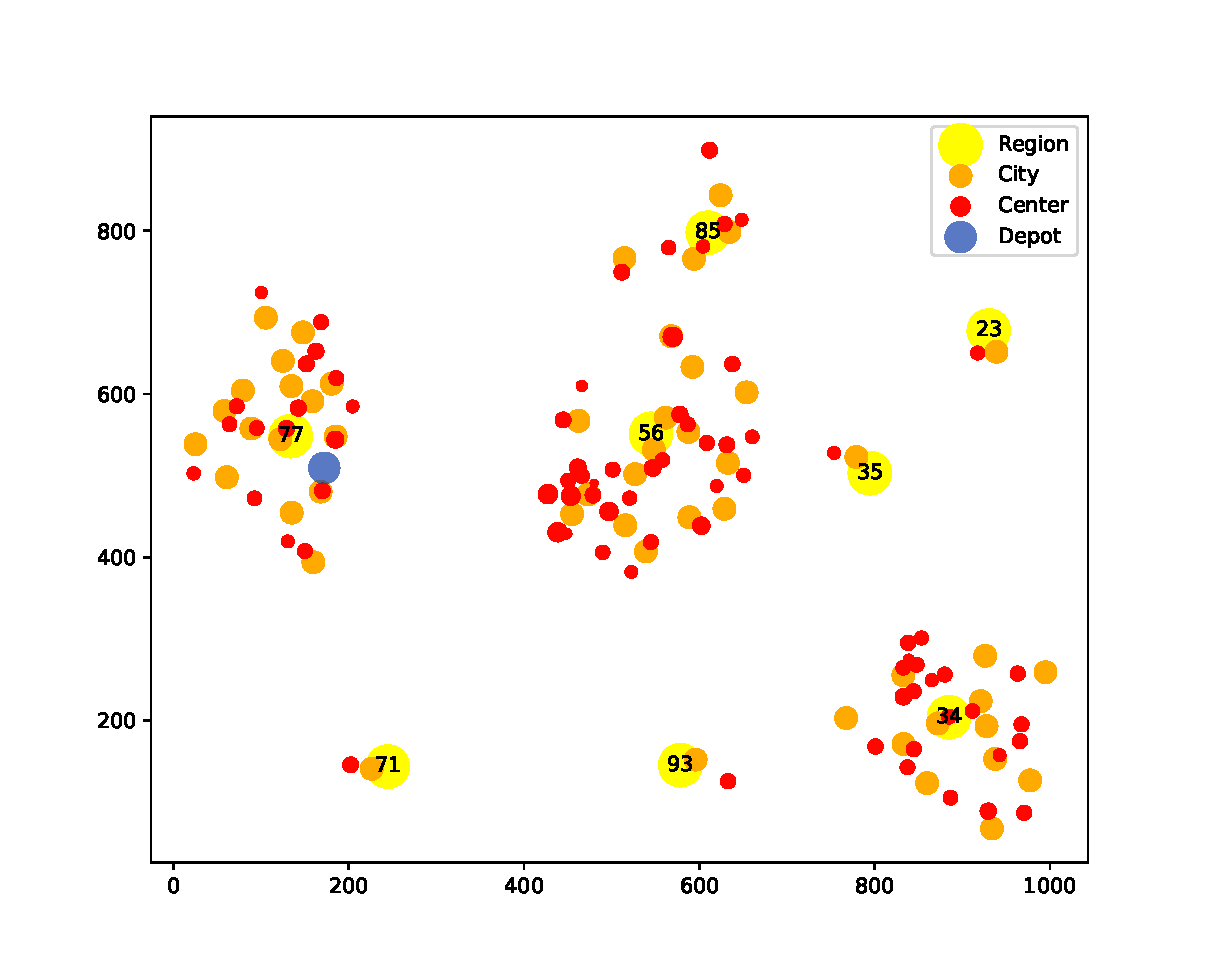
\includegraphics[width=1\columnwidth]{figures/center_locations.pdf}
    \caption{Locations of the centers in a square 2D grid}
  \label{fig:center_locations}
\end{figure}

\chapter{Vehicle Routing}
\label{vehicle-routing}
The final phase of our process is to determine the most efficient route for delivering the ingredients from the central depot to the delivery centers. We have modeled this problem as a Vehicle Routing Problem with Capacity constraints (VRPC). Given that there are 77 facilities, developing an optimal solution is a challenging task. As a result, we have explored three different solutions to address this issue. These include a polynomial approach, a method with subtour elimination, and a third approach that uses column generation and a custom branch and price model.

Of particular note is that while most formulations are independent of the precision of the numbers, the column generation model has a subproblem of cost $\mathbb{O}(Q^2N^2)$ where Q is the maximum capacity of the vehicles, thus, to have faster subproblem iterations the granularity of the vehicle capacity has been reduced, a similar reason is also used for the granularity of the distance. To offer better comparison between the different methodologies, the same granularities have been applied to the polynomial and subtour-elimination approaches.

\section{Polynomial model}
\label{polynomial-model}
The first method that we explored is a polynomial approach, which was the most straightforward solution. Despite its simplicity, this method is effective at identifying a feasible route for delivering ingredients to the various delivery centers.

\begin{align*}
    \min \quad & \sum_{i,j}{d_{i,j}x_{i,j}}\\
    \textrm{s.t.} \quad
      &\sum_{i \ne j} {x_{i,j}} = 1 \quad \forall j \in V \tag{1}\\
      &\sum_{j \ne i} {x_{i,j}} = 1 \quad \forall i \in V \tag{2}\\
      &\sum_{i \ne 0} {x_{0,i} - x_{i, 0}} = 0 \tag{3}\\
      &c_0 = 0 \tag{4}\\
      &c_j - c_i \geq w_j - M(1 - x_{i,j}) \quad \forall (i,j) \in A | i \ne j \land j \ne 0 \tag{5}\\
      &c_i \leq Q \quad \forall i \in V \tag{6}\\
      &x_{i,j} \in \{0,1\} \\
      &c_{i} \in \mathbb{N} \\
\end{align*}

Where $w_i$ is the material need of node $i$, $d_{i,j}$ is the distance from node $i$ to node $j$, $V$ is the set of nodes and $A$ is the set of arcs. The variables are: $x_{i, j}$ that is 1 if and only if the arc from node $i$ to node $j$ is selected, and $c_i$ that contains the accumulated capacity at node $i$.
The model minimizes the total distance, constraints 1, 2 and 3 are the flow constraints, while inequality 4, 5 and 6 constrain the capacity of the vehicles.

Constriant 5 activates when the arc $(i, j)$ is selected and constrains the capacity of the new node, as the inequality can be rewritten as $c_j >= c_i + w_j$. When node capacities are positive this inequality also imposes cycle elimination as $c_i$ must be strictly monotonic along the path.

\section{Subtour elimination model}
\label{subtour-elimination-model}
The second tested model is based on subtour elimination, also known as row generation. The general idea is that the model has a polinomial number of variables but an exponential number of constraints that are added incrementally during the exploration of the solution space. Usually the solution does not need to generate too many constraints, rendering this methodology usually faster than a polynomial formulation.

% TODO: multiple alignment (to align foralls)?
\begin{align*}
    \min \quad & \sum_{i,j \in A}{d_{i,j}\sum_{k \in K}{x_{i,j,k}}}\\
    \textrm{s.t.} \quad
      &x_{i,i,k} = 0 \quad \forall i \in V, k \in K \tag{1}\\
      &x_{i, 0, k} = 0 \quad \forall i \in V, k \in K \tag{2}\\
      &x_{n+1, i, k} = 0 \quad \forall i \in V, k \in K \tag{3}\\
      %
      &\sum_{j \in V,k \in K} {x_{i,j,k}} = 1 \quad \forall i \in C \tag{4}\\
      &\sum_{i \in C} {d_i\sum_{j \in V}{x_{i,j,k}}} <= Q \quad \forall k \in K \tag{5}\\
      % Flow constraints
      &\sum_{j \in V} {x_{0,j,k}} = 1 \quad \forall k \in K \tag{6}\\
      &\sum_{i \in V} {x_{i,n+1,k}} = 1 \quad \forall k \in K \tag{7}\\
      &\sum_{i \in V} {x_{i,h,k}} = \sum_{k \in V} {x_{h,j,k}} \quad \forall h \in C, k \in K \tag{8}\\
      % The exponential one
      &\sum_{(i, j) \in A} {x_{i,j,k}} \leq |S| - 1 \quad \forall S \subset V, k \in K \tag{9} \\
      &x_{i,j,k} \in \{0,1\} \\
\end{align*}

Here the nodes are a bit different than the previous model, node $0$ and $n+1$ are the depot node, and while $C$ is the set of customers ($n = |C|$), $V$ is the set of all nodes ($V = C \cup \{0, n+1\}$). The other used set is $K$ the set of usable vehicles, while $Q$, as in the other models is the maximum capacity for each vehicle. In this formulation we have only one three-dimensional variable, $x_{i,j,k}$ that is 1 if and only if vehicle $k$ uses the arc $(i,j)$.

The first three ineqaulities are just to remove unwanted arcs, 1 is to avoid 1-cycles, 2 and 3 remove cycles in and out of source and sink nodes. Constraint 4 allows each customer to be visited and cosntraint 5 limits the capacity for each vehicle. Flow constraints are enforced through ineqaulities 6 to 8.

The last constraint purpose is to remove cycles in each tour, but needs to be enforced for each possible cycle. To render this efficient we relax the problem and only add the constraints encountered when the problem solution contains cycles.

We adopted two additional details to increase the model performance: the first optimization is to use lazy constraints to speed up the optimization. The second one is less obvious, when a cycle is found we do not only remove that cycle but we remove the cycle also with the other $k$ (the other vehicles), this speeds up by a lot the convergence, otherwise the algorithm would try the same cycle with another vehicle.

\section{Column generation model}
\label{column-generation-model}

Column generation is a more complex approach, as such we have implemented the method described by Desrochers, Desrosiers and Solomon~\cite{desrochers1992new} simplified to remove time constraints and with a custom subproblem solution.

\begin{align*}
  \min \quad & \sum_{r \in R}{c_rx_r}\\
  \textrm{s.t.} \quad
    &\sum_{r \in R} {a_{i, r}x_r} \geq 1 \quad \forall i \in C \tag{1}\\
    &\sum_{r \in R} {x_r} = X_d \tag{2}\\
    &\sum_{r \in R} {c_rx_r} = X_c \tag{3}\\
    &x_{r} \in \{0,1\} \\
    &X_d, X_c \geq 0, integer.\\
\end{align*}


$C$ is the set of customers while $R$ is the set of all possible routes, in this model the $R$ set grows exponentially with the number of clients.

The variable $x_r$ is 1 iff the route is used, $X_d$ is the number of vehicles used and $X_c$ is the total distance traveled. Parameter $c_r$ is the total cost of route $r$ and $a_{i, r}$ counts how many times customer i is visited by route r. The system imposes integrality on the distance traveled, as such, the weights of the arcs should be integral too. To maintain precision while performing distance integralization, we defined a distance granularity parameter.

Constraint 1 requires all customers to be statisfied, while constraints 2 and 3 constrain the variables $X_c$ and $X_d$ to adhere to their definition, these are useful in the Branch and Price phase.

To resolve this problem without using an exponential number of variables, the system is first relaxed of its integrality constraints, and is then initialized with a feasible set of variables. After that the linear problem is solved and the dual variables are used to find better routes to add as variabels. This process is repeated until an optimal solution for the relaxed problem is found. To then find the integral solution another method called Branch and Price is required.

\subsection{Initial routes}
There are various strategies to select initial routes, one possible solution is to select the Identity matrix, interpreted as using one vehicle to visit each customer, while this does work it leads to inefficient first steps and additional subproblem cycles.
In this implementation the initial routes are selected with a custom heuristic that explores the closest nodes until the vehicle is filled, the pseudocode is written in Algorithm~\ref{alg:initial_routes}
\begin{algorithm}[htb]
  \caption{Algorithm to find an initial solution}\label{alg:initial_routes}
  \begin{algorithmic}
    %\Input{C set of customers, $d_{i,j}$ distance of nodes, $m_i$ material required by customer i}
    \State $routes \gets \{\}$
    \State $visited \gets \{\}$
    \State $current\_node \gets 0$
    \State $current\_route \gets \{\}$
    \State $current\_capacity \gets 0$

    \While{there are still nodes to visit}
      \State $n \gets closest\_unexplored\_node(current\_node)$
      \State {Add n to visited}
      \If{$current\_capacity + m_n \geq Q$}
        \State{Close path and add it to routes}
      \EndIf
      \State {Add $n$ to $current\_route$}
      \State $current\_node \gets n$
      \State $current\_capacity \gets current\_capacity + m_n $
    \EndWhile

    \State{Close the last path and add it to routes}
  \end{algorithmic}
\end{algorithm}


\subsection{Subproblem}
The used subproblem is a variation of what was described in the original paper, we revisited it to remove the time constraints and to be more intuitive.

Given the reduced costs of each arc: $\overline{c}_{i,j} = (1 - \pi_c)c_{i,j} - \pi_i$ where $\pi_0 = \pi_d$, the subproblem requires to find negative cost routes (from the depot back to the depot) with capacity constraints traversing the graph. The graph can also contain negative loop cycles, making the problem NP hard in the strong sense.

Our solution is a simple Dynamic Programming algorithm similar to the Pulling Algorithm described in the paper, of complexity $\mathbb{O}(Q^2N^2)$
\begin{align*}
  &C_0(0) = 0 \\
  &C_j(q) = \min_{i \in V} \{G_i(q\prime) + \overline{c}_{i,j} | q\prime + q_j \leq Q\}
\end{align*}

This computes the minimal paths for each of the nodes, available in $C_i(Q) \forall i \in V$.

In addition to this the implementor will want to keep a predecessor matrix to keep track of the real computed route. This also helps in determining the 2-cycle elimination algorithm, the idea is to keep track of the best two routes for each state, one that is the best route, and the second one that is the best route using a different predecessor node.

\begin{align*}
  C_0(0) = 0 \\
  &P_j(q) = arg\,min_{i \in V} \{
    [C_i(q^\prime) + \overline{c}_{i,j} \text{if} j \neq P_i(q), C^\prime_i(q^\prime) + \overline{c}_{i,j}] |
    q^\prime + q_j \leq Q
  \} \\
  &C_j(q) = C_{P_j(q)} + \overline{c}_{i,P_j(q)} \\
  &C^\prime_j(q) = \min_{i \in V} \{
    [C_i(q^\prime) + \overline{c}_{i,j} \text{if} j \neq P_i(q), C^\prime_i(q^\prime) + \overline{c}_{i,j}] |
    q^\prime + q_j \leq Q \land i \neq P_j(q)
  \}
\end{align*}

A simple interpretation of this algorithm is that $C_i(q)$ offers the best route to arrive at node i with node capacity q, $C^\prime_i(q)$ offers the second best route and $P_i(q)$ contains the predecessor node to obtain $C_i(q)$. In a real algorithm $P^\prime_i(q)$ should also be computed to reconstruct the real paths. $C_i(q)$ selects the best paths using capacities less than $q - q_j$, also checking that the path doesn't to 2-cycles. By iterating the problem with every node at every capacity we obtain the minimal route to arrive at each node.

The subproblem is a critical component of the algorithm as it is where the model will spend most of the time, to have faster iterations we implemented the subproblem using Cython~\cite{behnel2011cython}, while all of the other project is developed using Python. This alone has achieved a 10x speedup for the solution of every subproblem.

Since the complexity of the subproblem higly depends on $Q$, the maximum capacity for each vehicle, as a speed optimization we offer a capacity granularity, by having less granularity the results are less precise but the subproblem speed decreases quadratically. All of the results have a capacity granularity of 1000 Kg per customer where $Q = 10000Kg$.

\subsection{Branch and Price}
The Branch and Price algorithm is the same as described in the original algorithm, we implemented some optimizations to deduplicate paths and other minor implementation details. The exploration direction in the algorithm is parametrized but by default a mixed exploration is selected as it quickly arrives at an integral solution and it keeps the number of unexplored nodes comparatively low.

Developing a Branch and Price technique is quite error-prone for a student, as such we integrated a debug mode that enables exploration of the Branch and Price tree after the optimal solution has been found, keeping track of the Gurobi model and added constraints. This online debugging strategy has been a helpful way to locate and remove multiple coding mistakes.

\chapter{Results}
\label{results}
In this chapter we will present the results and offer a possible interpretation.

\section{Preface}
While the problem instance is too big to find an optimal solution, the models have been given ample time to compute feasible qualitative routes. Unexpectedly, the subtour elimination model is less efficient than the polynomial model, even in smaller instances. Even more unexpectedly, the polynomial formulation seems to be more efficient than the custom Column Generational approach, finding better solutions in orders of magnitude less time.

We have run the models on two datasets each: one using the forecasted data and the other using the real data.
The polynomial and subtour elimination models have been time-limited by the memory of the calculator, they seem to consume far more than what the running computer had to offer, thus their times are lower than those for column generation.


\section{Data}
The data collected by running each of the models can be summarized in the following table, we remind that the models were not run to conclusion but were limited by the capabilities of the available machine.

\begin{tabular}{ |p{2cm}||p{1.5cm}|p{1cm}|p{1.6cm}|p{1.4cm}|p{1,5cm}|p{1.5cm}|p{1.7cm}|  }
  \hline
  Model & Data & Time & Upper Bound & Lower Bound & Initial Lower Bound & Explored nodes & Generated Columns /Rows \\
  \hline
  Col. Gen. & Forecast & 11h & 12275.91 & 10653.04 & 10624.35 & 192295 & 302000 \\
  Col. Gen. & Real & 22h & 11456.74 & 10573.27 & 10549.30 & 363886 & 766420 \\
  Poly. & Forecast & 8h$^\dagger$ & 11223.83 & 4794.40 & 4034.81 & 4977643 & - \\
  Poly. & Real & 5h$^\dagger$ & 11354.86 & 4761.03 & 4033.18 & 4670016 & - \\
  Sub. Elim. & Forecast & 4h$^\dagger$ & 40474.66 & 4146.30 & 3931.12 & 141979 & 19452 \\
  Sub. Elim. & Real & 4h$^\dagger$ & 40474.66 & 4204.66 & 3931.12 & 138154 & 19473 \\
  \hline
\end{tabular}

We highlighted with $\dagger$ the models that had to be terminated for memory scarcity.

The best routes computed by the polynomial and column generation models at their time of termination are displayed in Figure~\ref{fig:res-colgen-avg}, Figure~\ref{fig:res-colgen-real}, Figure~\ref{fig:res-poly-avg} and Figure~\ref{fig:res-poly-real}. The subtour elimination approach did not generate intermediate results, as such it is impossible to find a comparable route.

The unprocessed information we used to compute summaries and visualizations can be found in the "logs" folder provided with the project.

\section{Discussion}
As can be observed, the polynomial model consistently yields superior results in significantly less time compared to our Branch and Price method. This observation is a testament to the impressive work done by the Gurobi team in developing Mixed Integer Programming (MIP) solving solutions that can efficiently handle even the most straightforward problem formulations.

It is worth noting, however, that we may have achieved even better results had we implemented more efficient subproblem formulations. With the benefit of hindsight, we recognize that given the number of clients required, a metaheuristic solution might have been a more appropriate approach. Nonetheless, the results obtained through our selected approach provide valuable insights into the problem and pave the way for further optimization efforts in the future.



\begin{figure}[tb]
    \centering
    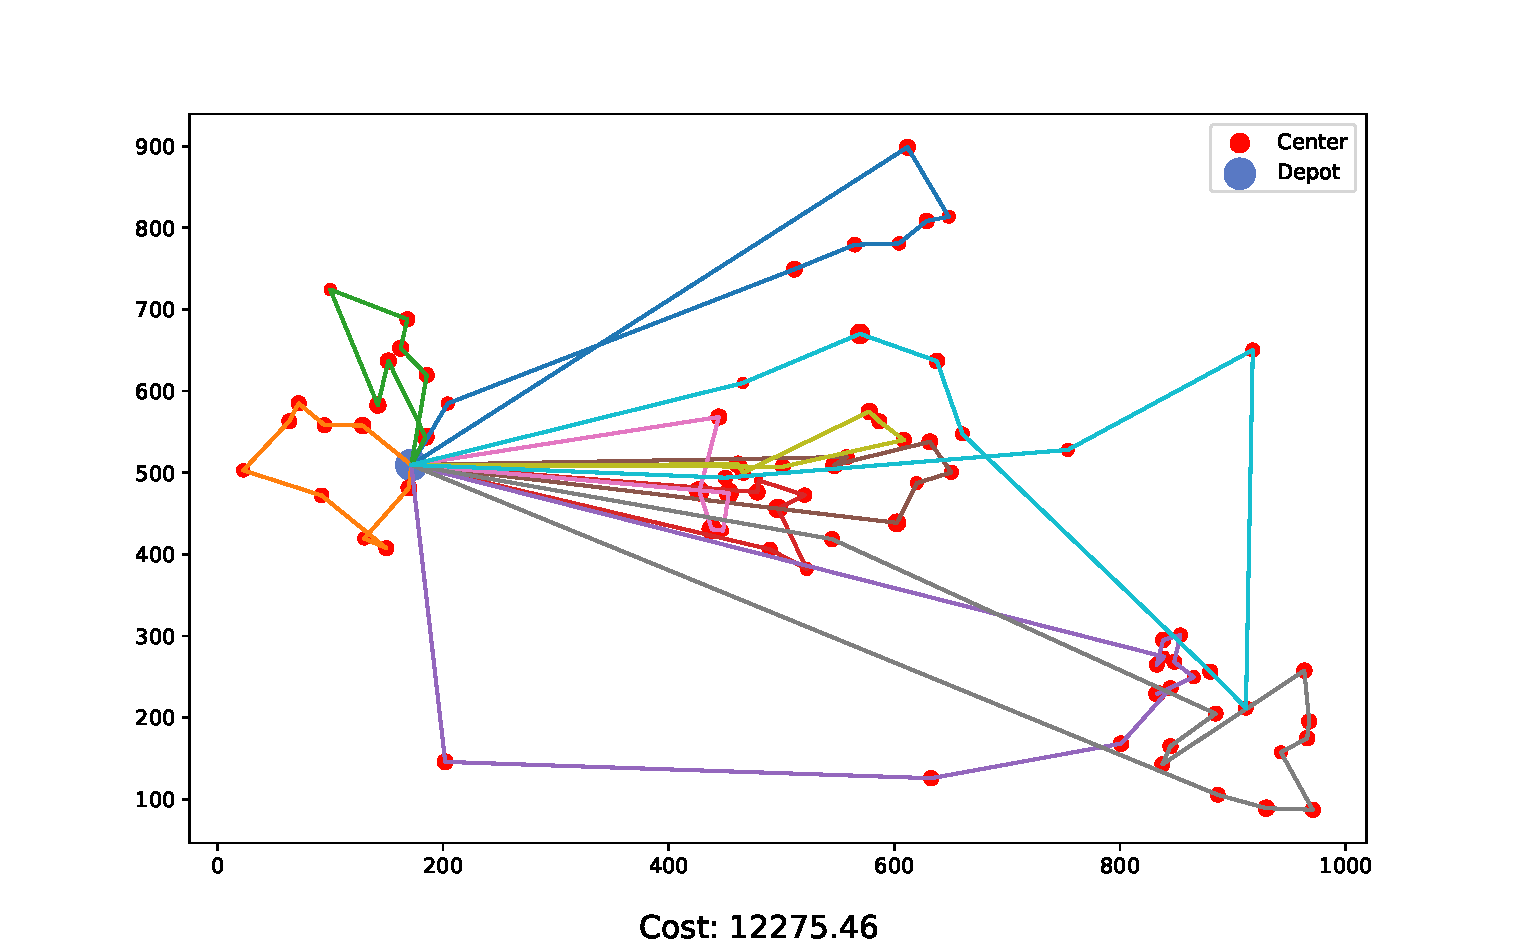
\includegraphics[width=1\columnwidth]{figures/results_colgen_avg.pdf}
    \caption{method: column generation, data: average, runtime: 11h}
  \label{fig:res-colgen-avg}
\end{figure}

\begin{figure}[tb]
    \centering
    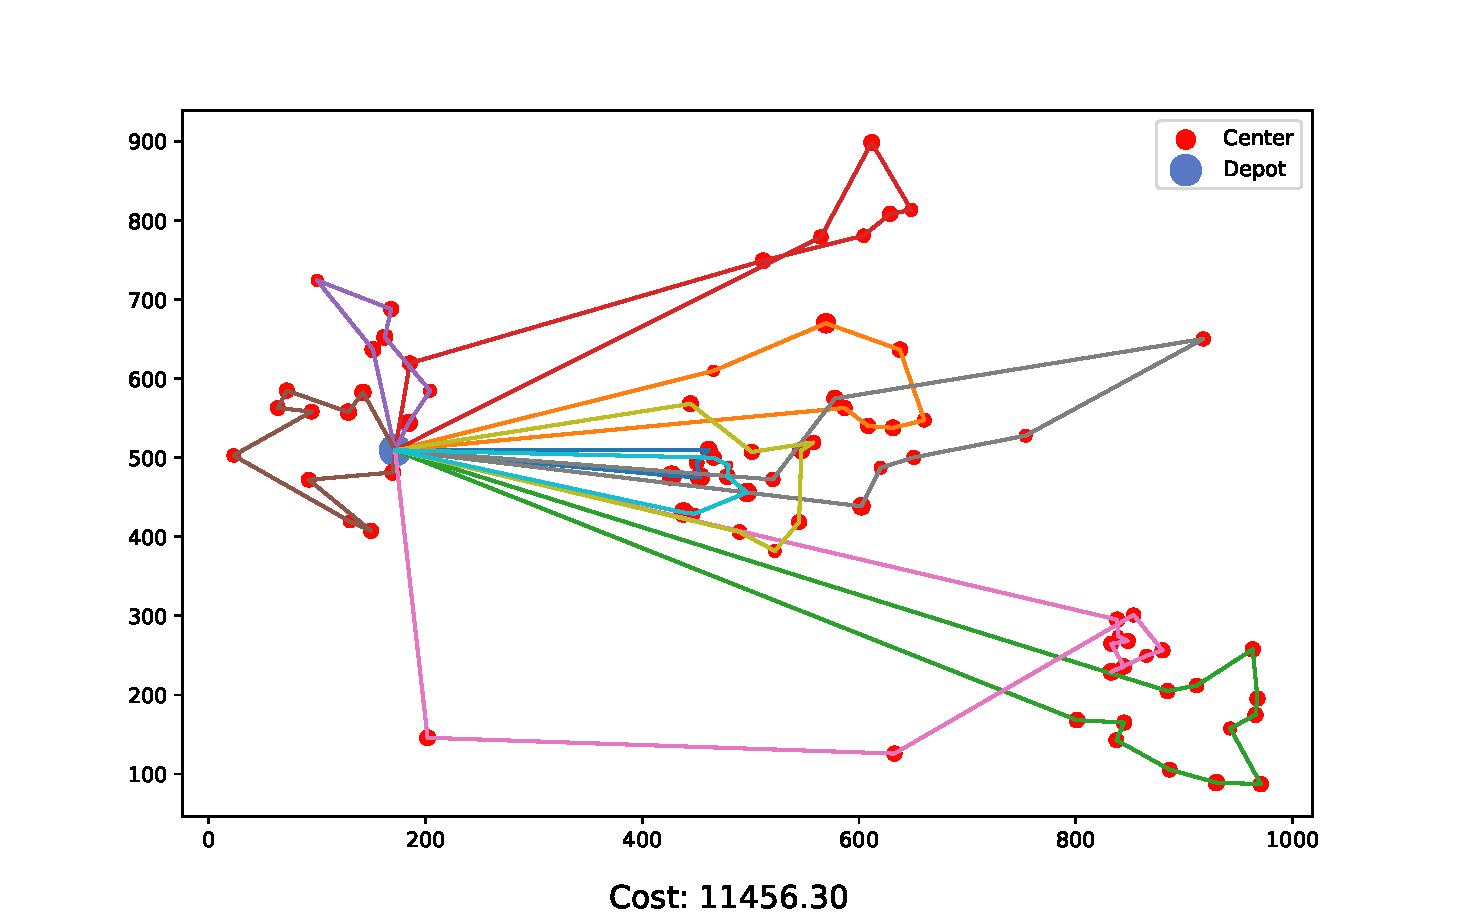
\includegraphics[width=1\columnwidth]{figures/results_colgen_real.pdf}
    \caption{method: column generation, data: real, runtime: 22h}
  \label{fig:res-colgen-real}
\end{figure}

\begin{figure}[tb]
    \centering
    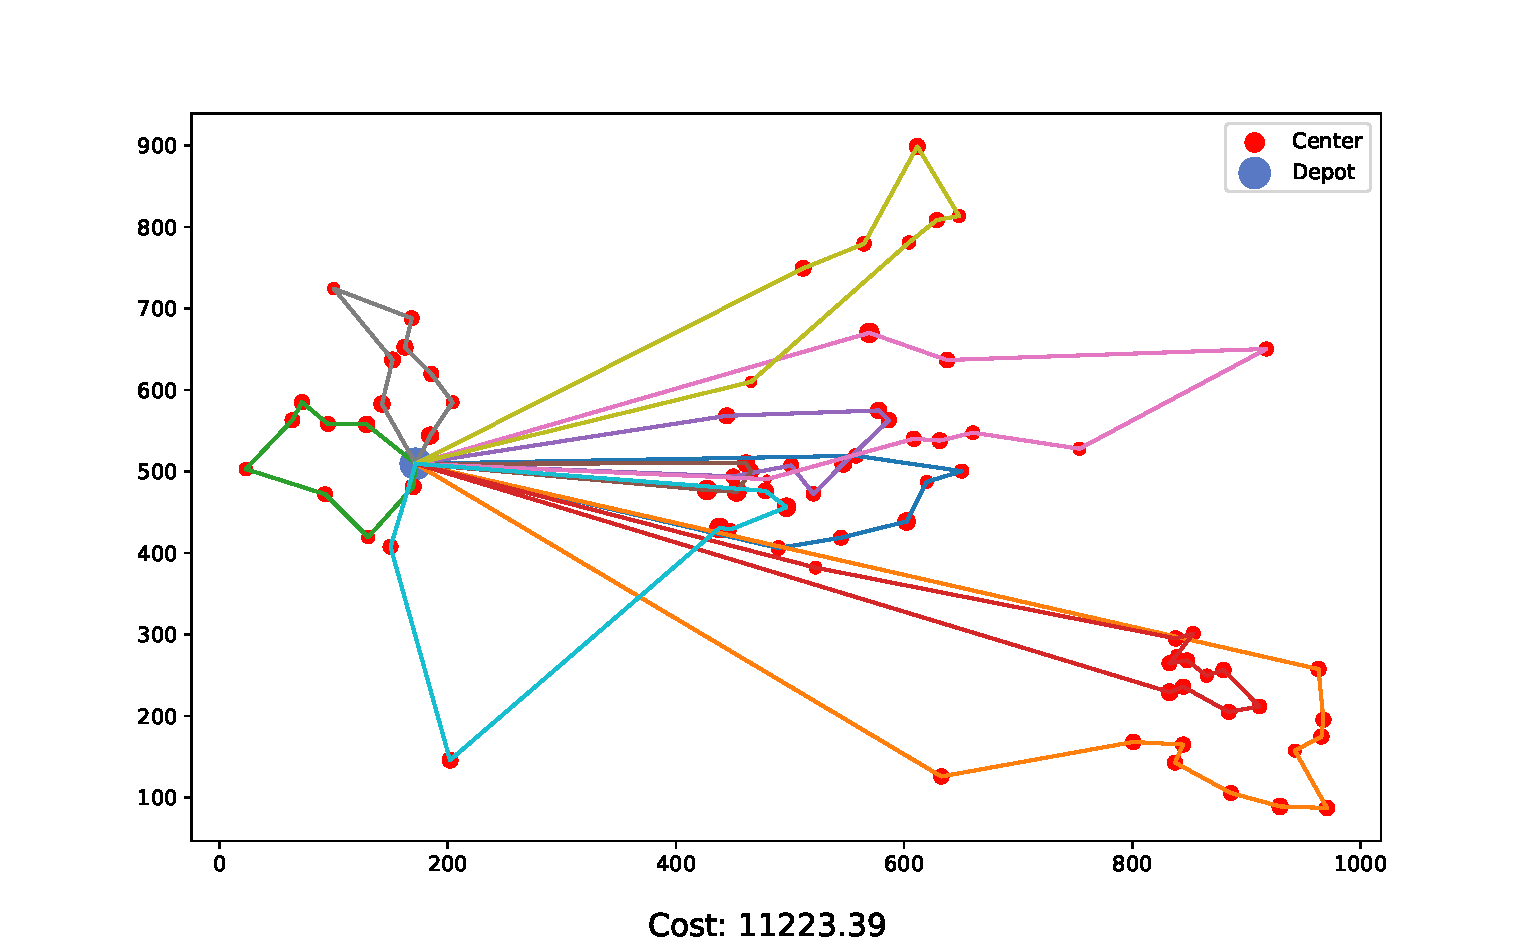
\includegraphics[width=1\columnwidth]{figures/results_poly_avg.pdf}
    \caption{method: polynomial, data: average, runtime: 7h}
  \label{fig:res-poly-avg}
\end{figure}

\begin{figure}[tb]
    \centering
    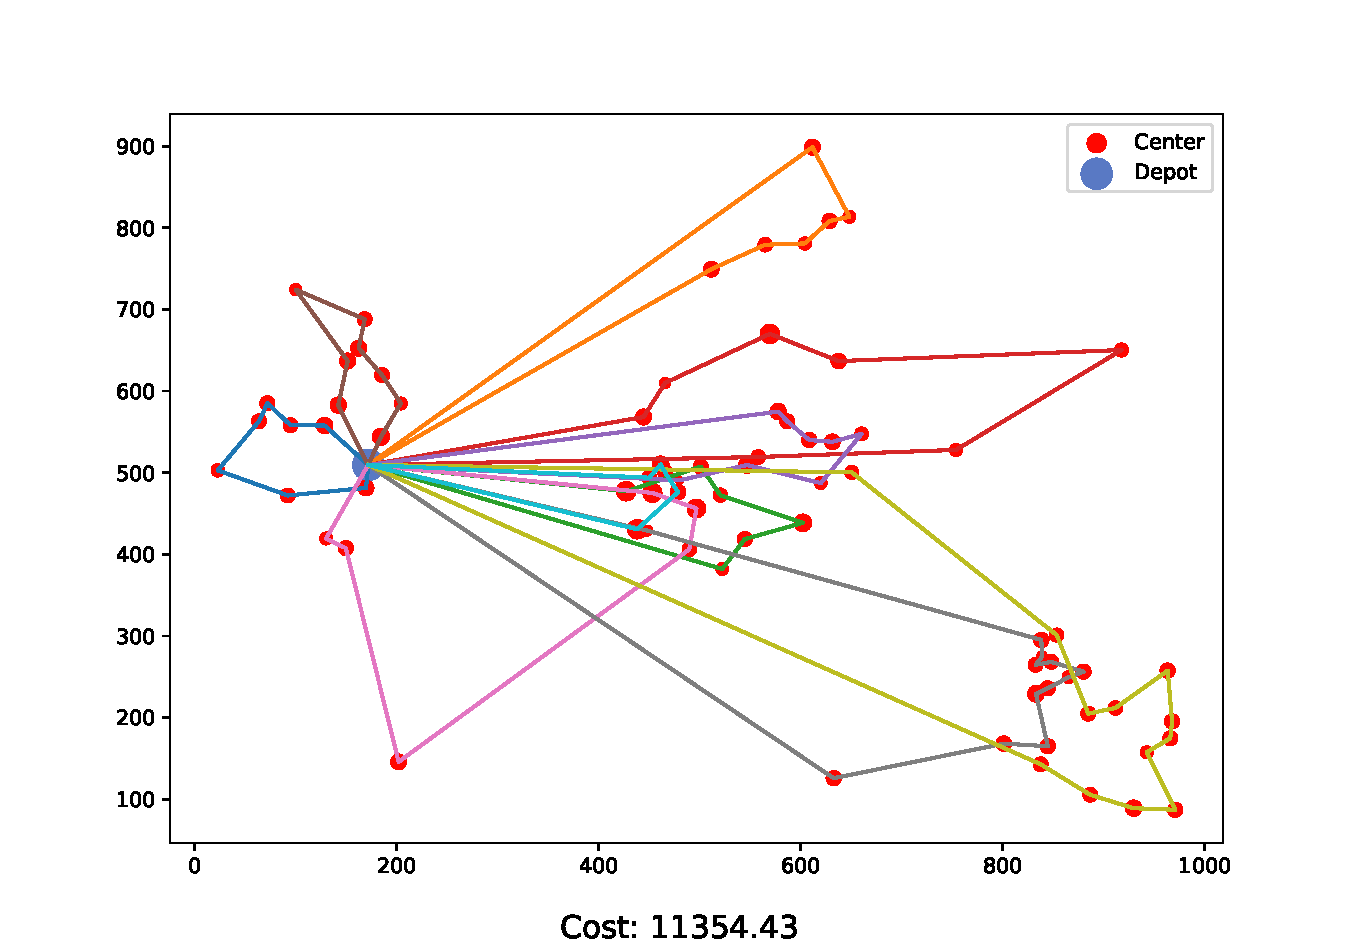
\includegraphics[width=1\columnwidth]{figures/results_poly_real.pdf}
    \caption{method: polynomial, data: real, runtime: 5h}
  \label{fig:res-poly-real}
\end{figure}



\begin{flushleft}
\bibliographystyle{plain}
\bibliography{sections/references}
\end{flushleft}

\end{document}
